\documentclass[11pt]{article}
\usepackage[T1]{fontenc}
\usepackage{lmodern,microtype,amsmath,amssymb,amsthm,mathtools,mathrsfs,xurl}
\usepackage[a4paper,margin=28mm]{geometry}
\usepackage{tikz}
\usetikzlibrary{arrows.meta,positioning,calc}
\usepackage[colorlinks=true,linkcolor=blue!55!black,citecolor=blue!55!black,urlcolor=blue!55!black]{hyperref}
\setlength{\emergencystretch}{2em}
\numberwithin{equation}{section}
\newtheorem{theorem}{Theorem}[section]
\newtheorem{lemma}[theorem]{Lemma}
\newtheorem{proposition}[theorem]{Proposition}
\newtheorem{corollary}[theorem]{Corollary}
\theoremstyle{definition}\newtheorem{definition}[theorem]{Definition}
\theoremstyle{remark}\newtheorem{remark}[theorem]{Remark}
\newcommand{\ii}{\mathrm i}
\newcommand{\dd}{\,\mathrm d}
\newcommand{\Turn}{\mathcal T}
\newcommand{\Log}{\operatorname{Log}}
\newcommand{\diag}{\operatorname{diag}}
\newcommand{\Vol}{\operatorname{Vol}}
\title{Holomorphic source asymptotics and volume limits\\for strict Conway compositions}
\author{}\date{}
\begin{document}
\maketitle
\begin{abstract}
We prove a nonzero asymptotic for the entire filling evaluation of a fixed strict Conway composition with at least two crossing circles. The auxiliary filling integers are independently signed and sufficiently long, and are fixed before the level tends to infinity. Exact factorial interpolation of the pure source gives a holomorphic stationary action at every strict leaf index. Two finite lattice saddles retain the original integer offsets and give nonzero amplitudes at both parities. Expanding each full physical crossing power into ordinary circles puts the actual filling under a real-action whole-period theorem. A classical shear identity identifies its critical value with the volume of the original primitive filling, including odd crossing powers. We also retain a separate signed-leaf interpolation and signed source expansion for the completed-root subfamily. The enlarged volume theorem uses the pure source and does not require that additional signed expansion.
\end{abstract}

\section{The construction, the asymptotic and the inputs}\label{ca:intro}

An elementary box $h$ is the physical quarter-turn of a circle surrounding two main strands. Every occurrence has its own auxiliary circle, punctured disk and original disk framing. Form an ordered expression from distinct copies of $h$, products and clockwise physical quarter-turns $\Turn$, and close it as $C(FG)$.
Endpoints are numbered $0,1,2,3$ cyclically from the bottom left. In a product with $F$ below $G$, join $F_2$ to $G_1$ and $F_3$ to $G_0$; the exposed tuple is $(F_0,F_1,G_2,G_3)$. A turn replaces a tuple by $(C_1,C_2,C_3,C_0)$, moving the entire box and its disks. Cylindrical closure joins $0$ to $3$ and $1$ to $2$.

The expression is \emph{strict} if its original wire constraints have a state with leaf labels $0<a<1/2$, turn relation $x\mapsto1-x$, and
\[
                \max(x,y)<z<x+y<1
\]
at every product below the closing root. At the root the two outputs are complementary; its forced product is removed. This is the finite type condition of \cite[Lemma 2.2]{Profiles}. Strictness concerns this particular presentation, including its turns. It allows an elementary or turned elementary child at the closing root.

Fix such an expression with $b\ge2$ circles. At circle $\ell$ retain $\epsilon_\ell\in\{0,1,-1\}$ half twists and fill the original primitive slope $\mu_\ell+p_\ell\lambda_\ell$, where $\mu_\ell$ is its meridian and $\lambda_\ell$ its disk longitude. The physical crossing power is
\begin{equation}\label{ca:n}
 n_\ell=\epsilon_\ell-2p_\ell.
\end{equation}
Assume the actual main-strand diagram after these retained half twists has exactly one component. This test counts any component closed inside a product as well as the final endpoint closure. Full twists preserve every endpoint connection and internal component, so the resulting main link is a knot $K_{\epsilon,\mathbf p}$. The circles and their fillings are those of the original construction; they are not substituted by a different surgery presentation.

At level $N\ge3$ put $d=N-1$, $q=e^{\pi\ii/N}$ and
$\kappa=q^{d^2/2}$, with $q^t=e^{\pi\ii t/N}$. Let $D$ be the oriented blackboard diagram of the filled knot, and let $w(D)$ denote its writhe. The actual reduced tensor evaluation is corrected to zero framing by
\begin{equation}\label{ca:framing}
 \zeta_{N,D}=\theta^{-w(D)},\qquad
 \theta=q^{-d^2/2}=\kappa^{-1}.
\end{equation}
For another explicitly specified ribbon framing one uses that integer framing correction instead. The single reduced cut has unknot value one. Its identification with the reduced Kashaev invariant is \cite[Theorem 10.1]{Finite}; no additional factor is assigned to an auxiliary circle.

The pure complete source has a unique strict stationary state. Write its value as $F_0$ and its leaf coordinates as $a_\ell$. The boundary parameters
\[
 X_\ell=\cot(\pi a_\ell)>0
\]
are defined at the strict optimizer of \cite[Theorem 3.3]{Profiles}. No lower bound $a_\ell>1/4$ is required for the main theorem. Section~\ref{ca:strict-pure-section} constructs the holomorphic pure-color critical action $\Phi_0(t)$ with $\Phi_0(0)=F_0$. Its Fourier Legendre action is
\begin{equation}\label{ca:Psi}
 \nabla\Phi_0(\xi(z))+2\pi\ii z=0,\qquad
 \Psi_0(z)=\Phi_0(\xi(z))+2\pi\ii\,\xi(z)\cdot z.
\end{equation}
All these germs are fixed by their complete values and the original logarithmic branches.

\begin{theorem}[The entire filled evaluation]\label{ca:main}
For every fixed strict construction with $b\ge2$ and retained half-twist pattern satisfying the stated knot test, there is $P_0$ such that the following holds for every fixed signed integer tuple with $|p_\ell|>P_0$ for every $\ell$. The phase
\[
 T_{\mathbf n}(z)=\Psi_0(z)+\pi\ii\sum_{\ell=1}^b n_\ell z_\ell^2
                           +2\pi\ii\sum_{\ell=1}^b z_\ell
\]
has a unique critical point $z_{\mathbf n}$ near zero. Put
$S_{\mathbf n}=T_{\mathbf n}(z_{\mathbf n})$ and
$Q_{\mathbf n}=-T_{\mathbf n}''(z_{\mathbf n})$. There is a holomorphic nonzero Fourier amplitude $B$ near zero, defined in \eqref{ca:Fourier-amplitude}, such that
\begin{align}
 K_N(K_{\epsilon,\mathbf p})
 &=\zeta_{N,D}\,\kappa^{\frac12\sum_\ell n_\ell}
 N^{3/2}D(\mathbf n)e^{NS_{\mathbf n}}
 \bigl(1+O_{\mathbf p}(N^{-1})\bigr),\label{ca:asymptotic}\\
 D(\mathbf n)&=
 \frac{(-2\ii)^b(2\pi)^{b/2}B(z_{\mathbf n})
       \prod_\ell\sin(2\pi z_{\mathbf n,\ell})}
      {\sqrt{\det Q_{\mathbf n}}}\ne0.\label{ca:D}
\end{align}
The square root is the Gaussian branch with positive real quadratic form. The formula holds through all sufficiently large integer levels, with both parities and composite levels included. In particular the invariant is eventually nonzero and
\begin{equation}\label{ca:volume}
 \lim_{N\to\infty}\frac{2\pi}{N}\log|K_N(K_{\epsilon,\mathbf p})|
 =2\pi\Re S_{\mathbf n}
 =\Vol(S^3\setminus K_{\epsilon,\mathbf p}).
\end{equation}
There is no bound on the ratios or relative signs of the filling integers. They do not grow with $N$.
\end{theorem}

The exact Newton turn, trace, multiplication, circle split and crossing polynomial are \cite[Proposition 3.2, Theorem 3.3, Proposition 4.1 and equation (4.8)]{Newton}. These finite local identities apply to the original expression. The enlarged variational inputs are \cite[Lemma 3.1 and Theorem 3.3]{Profiles}: primitive wire coordinates, a unique strict maximum and its negative definite Hessian. Theorem 1.1 of \cite{Bounds} controls the entire complementary source and every physical color a fixed fraction below complete color when $b\ge3$; its Corollary 9.1 supplies exactly these conclusions when $b=2$. We use both with all retained signs set to zero.

Theorem 1.1 of \cite{Filling} evaluates an exact periodic polynomial filling source after its real local action and shared global gap have been proved. Theorem 1.3 of \cite{StrictGeometry} constructs the original primitive fillings and their absolute metric volume for this same strict syntax. Its classical potential is defined directly from cells. We will identify it with the pure source action by an explicit shear, without importing a signed quantum expansion at a quarter-index leaf.

For a separate local result we retain the \emph{completed-root} grammar of \cite[Definition 2.1]{Newton}: a completed box starts with a stack of two elementary pieces and is built by turns, stacks of completed boxes and attachment of an elementary piece to a completed box; both closing boxes are completed. Its stationary leaves lie above $1/4$. Section~\ref{ca:leaf} and Theorem~\ref{ca:packet-theorem} prove the signed local coefficient and source expansions in that scope. Theorem~\ref{ca:strict-pure} then proves the pure source expansion for every strict expression independently of those signed estimates.

There is a useful distinction in applying the filling theorem. A source with retained half twists has a complex local phase even at real color. The real-action hypothesis of \cite{Filling} cannot simply be assigned to it. We instead expand the full physical integer power $R^{n_\ell}$ at each disk into ordinary circles before taking any asymptotic limit. This finite identity uses the pure source and preserves the actual knot. An odd power in that algebraic expansion is not interpreted as a half-integral Dehn filling of the pure augmented partner: the final geometric comparison uses the original retained half twist and the integer $p_\ell$ in \eqref{ca:n}.

\section{A normalized factorial on a complex strip}\label{ca:factorial-section}

We first fix the interpolation used in every subsequent contour. Put
$Q=e^{2\pi\ii/N}$ and
\[
 S_r=\prod_{j=1}^r2\sin(\pi j/N),\qquad S_0=1.
\]
The function below is a normalized solution of a sine difference equation. Only the ordinary Gamma functional equation, its Stirling expansion with remainder, and the convergent sine product are needed; the standard Gamma formulas are recorded in \cite[\S\S5.5(i), 5.11(i)--(ii)]{DLMF}.

\begin{lemma}[Canonical factorial interpolation]\label{ca:factorial}
For $N\ge2$ and $-1<\Re z<N$ the product
\begin{equation}\label{ca:G}
 G_N(z)=\left(\frac{2\pi}{N}\right)^z\Gamma(z+1)
 \prod_{k=1}^{\infty}
 \frac{\Gamma(Nk+z+1)}{\Gamma(Nk-z)(Nk)^{2z+1}}
\end{equation}
is holomorphic and nonzero. Positive-base powers use their real logarithms. With $d=N-1$ and
\[
 \widehat F_N(z)=e^{\pi\ii z(z+1)/(2N)-\pi\ii z/2}G_N(z)
\]
one has the exact identities
\begin{align}
 G_N(z+1)&=2\sin\!\frac{\pi(z+1)}N\,G_N(z),\notag\\
 \widehat F_N(z+1)&=(1-Q^{z+1})\widehat F_N(z),\label{ca:shift}\\
 G_N(0)&=1,\qquad G_N(r)=S_r,\qquad
 \widehat F_N(r)=(Q;Q)_r\quad(0\le r<N),\notag\\
 G_N(z)G_N(d-z)&=N,\notag\\
 \widehat F_N(z)\widehat F_N(d-z)&=
 N e^{\pi\ii z(z-d)/N}.\label{ca:reflection}
\end{align}
Identities are asserted where the factors are regular, and elsewhere by meromorphic continuation. If
\[
 H_N(s)=\prod_{j=1}^{d}
       \frac{\sin(\pi(j-s)/N)}{\sin(\pi j/N)}
       =\frac{\sin(\pi s)}{N\sin(\pi s/N)},
\]
then on $|s|<1$,
\begin{equation}\label{ca:small-reflection}
 G_N(s)G_N(-s)=H_N(s)^{-1}.
\end{equation}

Let $J$ be the analytic primitive of $\Log(2\sin\pi x)$ on
$0<\Re x<1$, fixed by its integrable limit $J(0)=0$ along the real interval. On every compact subset of this strip,
\begin{equation}\label{ca:Stirling}
 \log G_N(Nx)
 =NJ(x)+\tfrac12\Log(2N\sin\pi x)
       +\frac{\pi\cot\pi x}{12N}+O(N^{-3}).
\end{equation}
The branches are real on $0<x<1$. More generally, for each fixed $L\ge1$ the correction is
\begin{align}
 &\sum_{r=1}^{L}\frac{c_{2r-1}(x)}{N^{2r-1}}+O(N^{-2L-1}),\notag\\
 &c_{2r-1}(x)=\frac{B_{2r}}{2r(2r-1)}
 \left\{x^{1-2r}+
 \sum_{k\ge1}\bigl[(k+x)^{1-2r}-(k-x)^{1-2r}\bigr]\right\}.
 \label{ca:all-Stirling}
\end{align}
Here $B_j$ are defined by $t/(e^t-1)=\sum B_jt^j/j!$.
All fixed derivatives have the same uniform remainder orders on smaller compact sets. Fixed bounded complex offsets are included by substituting $x+c/N$; in particular
\begin{equation}\label{ca:offset}
 G_N(Nx+c)=
 \sqrt{2N\sin\pi x}\,e^{NJ(x)}(2\sin\pi x)^c
 \bigl(1+O(N^{-1})\bigr).
\end{equation}
\end{lemma}

\begin{proof}
The logarithm of the $k$th factor in \eqref{ca:G} is
\[
 -\frac{z(z+1)(2z+1)}{6N^2k^2}+O(k^{-3})
\]
locally uniformly in $z$. The product and all its local logarithmic derivatives therefore converge. Its factors are nonzero in the stated strip and its value at zero is one. Gamma's functional equation gives
\[
 \frac{G_N(z+1)}{G_N(z)}
 =\frac{2\pi(z+1)}N
  \prod_{k\ge1}\left(1-\frac{(z+1)^2}{N^2k^2}\right)
 =2\sin\frac{\pi(z+1)}N.
\]
Multiplying by the displayed exponential gives the second shift. This also fixes the lattice values, including their phases.

To remove any periodic ambiguity in reflection, differentiate
$\log[G_N(z)G_N(d-z)]$. In the product truncated at $k=K$ the resulting sum telescopes to
\[
 \psi(NK+z+1)-\psi(N(K+1)-z),
\]
where $\psi=\Gamma'/\Gamma$. It tends locally uniformly to zero. The product is constant, and at $z=0$ it equals $S_d=N$. The latter equality follows by taking the absolute value of
$\prod_{j=1}^{N-1}(1-e^{2\pi\ii j/N})=N$.
This proves both formulas in \eqref{ca:reflection}, with the marked phase obtained by adding the two quadratic exponents. Iterating the shift from $-s$ to $d-s$ gives
$G_N(d-s)=N H_N(s)G_N(-s)$, which proves \eqref{ca:small-reflection}. The finite sine product gives the displayed quotient for $H_N$, with its removable value one at zero.

We give the remainder argument for \eqref{ca:Stirling}, because contours require a complex estimate rather than values on an integer mesh. Stirling's expansion on a closed right-half-plane sector has remainder $O(|w|^{-2L-1})$ after its term in $w^{1-2L}$. One obtains this bound from the Euler summation formula for $\log\Gamma$: the remaining periodic Bernoulli polynomial is bounded, and its integral is bounded by a constant times
$\int_0^\infty|w+t|^{-2L-2}\dd t$.
For $x$ in a fixed complex compact set as above, $Nx$ and
$N(k\pm x)$ lie in a common such sector.

For $L=1$ the logarithm of the $k$th factor in \eqref{ca:G}, at $z=Nx$, becomes
\[
 N\phi_k(x)+\tfrac12\Log(1-x^2/k^2)
 +\frac1{12N}\left(\frac1{k+x}-\frac1{k-x}\right)
 +O(N^{-3}k^{-3}),
\]
where
\[
 \phi_k(x)=(k+x)\Log(1+x/k)
 -(k-x)\Log(1-x/k)-2x.
\]
The remainder is summable. Moreover $\phi_k(0)=0$ and
$\phi_k'(x)=\Log(1-x^2/k^2)$. The sine product, including the
$\Gamma(Nx+1)$ factor, therefore sums the leading terms to $NJ(x)$.
It sums the half logarithms to $\frac12\Log(2N\sin\pi x)$.
The identity
\[
 \frac1x+\sum_{k\ge1}
   \left(\frac1{k+x}-\frac1{k-x}\right)=\pi\cot\pi x
\]
gives the first correction. Keeping further Stirling terms gives
\eqref{ca:all-Stirling}; their paired series converge locally uniformly, and the remainder sums absolutely as
$O(N^{-2L-1}\sum k^{-2L-1})$. The normalization of $J$, including its additive constant, was fixed by integration from zero, not by differentiation alone. Cauchy's formula on a larger compact set proves the derivative assertions. Taylor expansion at $x+c/N$ proves \eqref{ca:offset}.
\end{proof}

The reflection $J(1-x)=-J(x)$ follows by differentiating and using
$\int_0^1\log(2\sin\pi t)\dd t=0$. In particular $J(1/2)=0$. We will use
\[
 J(1/2+t)=-J(1/2-t)
\]
to normalize a sheared action at the actual terminal index.

\section{The actual high-index leaf and its shear}\label{ca:leaf}

A leaf index near the complete maximum belongs to a fixed compact interval
$I=[\tau_0,\tau_1]\subset(1/4,1/2)$. Throughout this section $x=r/N$ is that index and $t=h/N$ is the physical color deficit. We continue the color to a small complex disk; its radius is independent of $N$. Put
$M=\lfloor(N-1)/2\rfloor$ and $F_r=(Q;Q)_r$.

The finite Newton calculation of \cite[Proposition 4.1]{Newton} gives, for $r>h$,
\begin{align}
 A_N(r,t)&=\frac{N^2S_{2r}}
 {S_r^2G_N(r-Nt)G_N(r+Nt)},\label{ca:pure-leaf}\\
 d_N^\epsilon(r,t)&=\kappa^\epsilon
 \sum_{v=r}^M(-1)^v q^{\epsilon v(r+1)}
       \frac{S_v}{S_rS_{v-r}}A_N(v,t),
 \quad \epsilon=\pm1,\qquad d_N^0=A_N.\label{ca:signed-leaf}
\end{align}
Only the two color-shifted factorials are continued. The finite sum is therefore an exact even holomorphic function of $t$, with the original integer support. Set
$\ell_N^\epsilon=e^{-\pi\ii\epsilon d/4}d_N^\epsilon$.
This removes a constant unit phase, not a color-dependent phase.

\subsection{A recurrence with its physical upper endpoint}

For $h=Nt$ define
\begin{align}
 A_{h,r}&=\sum_{v=r}^M
 \frac{Q^{-vr}F_{2v}}
 {F_v\widehat F_N(v-h)\widehat F_N(v+h)F_{v-r}},\notag\\
 D_{h,r}&=\frac{Q^{-r^2}F_{2r}}
 {F_r\widehat F_N(r-h)\widehat F_N(r+h)},\qquad
 U_{h,r}=A_{h,r}/D_{h,r}.\label{ca:AU}
\end{align}
In the present corridor these denominators do not vanish. The last term gives $U_{h,M}=1$.

Put $Y=Q^r$, $H=Q^h=e^{2\pi\ii t}$ and $T=H+H^{-1}$. The exact recurrence is
\begin{multline}\label{ca:Ward}
 QY^2(1-Q^2Y)A_{h,r+2}
 +Y(TQ^3Y^2+Q+1)A_{h,r+1}\\
 -Q(QY+1)(QY^2-1)A_{h,r}=0,\qquad A_{h,M+1}=0.
\end{multline}
For clarity we verify the telescoping at complex color. The ratio of the $v+1$ summand to the $v$ summand, with $z=Q^v$, is
\[
 \frac{Y^{-1}(1-Qz^2)(1+Qz)}
 {(1-Qz/H)(1-QHz)(1-Qz/Y)}.
\]
Multiply by $g(z)=(1-z/H)(1-Hz)(1-z/Y)/z^2$ and take the forward difference. Dividing by the original summand leaves
\[
 \left(\frac1{YQ^2}-1\right)z^{-2}
 +\left(\frac1{YQ}+H+H^{-1}+\frac1Y\right)z^{-1}
 -\frac1{YQ}-1-\frac{H+H^{-1}}Y.
\]
Its lower endpoint vanishes because $z=Y$; its upper endpoint contains
$F_{2M+2}=0$. The index shift $r\mapsto r+1$ multiplies a summand by
$z^{-1}-Y^{-1}$. Expressing the two moments in these shifted sums and clearing denominators gives \eqref{ca:Ward}. This uses the exact shift of $\widehat F_N$, so it holds at complex $h$ without interpolation from finitely many colors.

Write $\operatorname{den}_r=(1-QY/H)(1-QYH)$. Division by the actual $D_{h,r}$ gives
\begin{align}
 U_r&=p_N(r,t)U_{r+1}+q_N(r,t)U_{r+2},\label{ca:recurrence}\\
 p_N&=-\frac{Q^{-2}Y^{-1}(TQ^3Y^2+Q+1)}
                 {\operatorname{den}_r},\notag\\
 q_N&=-\frac{Q^{-4}Y^{-2}(1-Q^2Y)(1-Q^3Y^2)(1+Q^2Y)}
                 {\operatorname{den}_r\operatorname{den}_{r+1}}.\notag
\end{align}
At $r=M-1$ one has
\begin{equation}\label{ca:wall}
 q_N(M-1,t)=0,\qquad U_{M-1}=p_N(M-1,t),\qquad U_M=1.
\end{equation}
For $N=2m+1$ the vanishing factor is $1-Q^3Y^2$, and for $N=2m$ it is $1+Q^2Y$. We have not divided by a nonexistent $D_{h,M+1}$.

\subsection{A holomorphic solution selected by that endpoint}

Regard $p_N,q_N$ as holomorphic functions of $(x,t,e)$ with
$e=1/N$, $Y=e^{2\pi\ii x}$ and $Q=e^{2\pi\ii e}$. Their leading terms are
\begin{equation}\label{ca:leading-pq}
 p_0=-Y^{-1}\frac{(H+H^{-1})Y^2+2}{D_t},\qquad
 q_0=-Y^{-2}\frac{(1-Y^2)^2}{D_t^2},\qquad
 D_t=(1-Y/H)(1-YH).
\end{equation}
At $t=0$ the roots of $\mu^2-p_0\mu-q_0=0$ are
\[
 \mu(x,0)=-Y^{-1},\qquad \mu_f(x,0)=Y^{-1}\cot^2(\pi x).
\]
On a compact interval in $(1/4,3/4)$ containing $[\tau_0,1/2]$, the first root has positive real part and
$|\mu_f/\mu|<1$. These inequalities persist uniformly on a fixed complex neighborhood and a small color disk:
\begin{equation}\label{ca:root-gap}
 \Re\mu\ge m_0>0,\qquad |\mu_f/\mu|\le k_0<1.
\end{equation}
In particular $\mu(1/2,t)=1$. Both $q_0$ and its first $e$ correction vanish there.

Choose $\sigma>0$ with
$[\tau_0-\sigma,1-\tau_0+4\sigma]\subset(1/4,3/4)$, and set
$L_N=\lceil(1/2-\tau_0+2\sigma)N\rceil$. For
$\mathcal F_x(w)=p(x,t,e)+q(x,t,e)/w$, define
\begin{equation}\label{ca:continued-fraction}
 v_N(x,t)=\mathcal F_x\circ\mathcal F_{x+e}\circ\cdots
 \circ\mathcal F_{x+(L_N-1)e}
       \bigl(\mu(x+L_Ne,t)\bigr).
\end{equation}
These compositions stay in disks of radius $Ce$ about the successive roots. Indeed one step has error $O(e)$ at the root and derivative at most $k_0+O(e)$. Taking $C$ larger than the error constant divided by $1-k_0$ makes the disks invariant, and they avoid zero. Thus $v_N$ is holomorphic and
$v_N=\mu+O(e)$, with all fixed derivative bounds on a smaller tube. On a physical grid point $x=r/N$, the composition passes through $M-1$. Equation \eqref{ca:wall} erases its artificial tail there. Backward substitution consequently gives the exact identity
\begin{equation}\label{ca:physical-ratio}
 v_N(r/N,t)=U_{h,r}/U_{h,r+1}\quad(r<M).
\end{equation}
This also proves that those actual coefficients do not vanish in the chosen complex color disk.

Write $p=p_0+ep_1+O(e^2)$ and $q=q_0+eq_1+O(e^2)$. Expanding one step gives
\begin{equation}\label{ca:nu}
 v_N=\mu+e\nu+O(e^2),\qquad
 \nu=\frac{p_1+q_1/\mu-q_0\mu_x/\mu^2}{1+q_0/\mu^2}.
\end{equation}
The denominator is $1-\mu_f/\mu$, separated from zero. The same contraction proves the error uniformly. Direct substitution at $t=0$ gives
\begin{equation}\label{ca:nu0}
 \Log\mu(x,0)=\pi\ii-2\pi\ii x,\qquad
 \frac{\nu(x,0)}{\mu(x,0)}
 =-\frac{\pi}{2}\cot(\pi x)-\frac{5\pi\ii}{2}.
\end{equation}
Define
\begin{align}
 S(x,t)&=\int_x^{1/2}\Log\mu(u,t)\dd u,\notag\\
 C(x,t)&=\sqrt{\mu(x,t)}
             \exp\!\int_x^{1/2}\frac{\nu(u,t)}{\mu(u,t)}\dd u.\label{ca:SC}
\end{align}
The logarithm is fixed by \eqref{ca:root-gap} and the square root by its value one at $1/2$. Ordinary Euler summation of \eqref{ca:physical-ratio} gives
$U_{h,r}=C(x,t)e^{NS(x,t)}(1+O(N^{-1}))$.
The physical endpoint $M/N$ differs from $1/2$ by $O(N^{-1})$; since
$\Log\mu(1/2,t)=0$, its missing integral contributes only $O(N^{-1})$ to the exponent. In particular no color-dependent constant is introduced at this endpoint. Formula \eqref{ca:nu0} gives
\begin{equation}\label{ca:SC0}
 S(x,0)=\pi\ii(1/2-x)^2,\qquad
 C(x,0)=\sqrt{\sin\pi x}\,
                  e^{-3\pi\ii(1/2-x)/2}.
\end{equation}

\subsection{Exponential accuracy before moving an index contour}

An error $O(N^{-1})$ on integer indices is insufficient when the sum of those indices has cancellation. We therefore construct an exponentially accurate interpolation of the same product. Let
$f_N=\Log v_N$ and $b_N=M/N$. On a fixed larger tube
$|f_N^{(j)}|\le B j! a^{-j}$ by Cauchy's formula. Choose a sufficiently small constant $c>0$ and put $K_N=\lfloor cN\rfloor$. Set
\begin{align}
 E_N(x,t)={}&N\int_x^{b_N}f_N(u,t)\dd u
       +\tfrac12\{f_N(x,t)-f_N(b_N,t)\}\notag\\
 &+\sum_{k=1}^{K_N}\frac{B_{2k}N^{1-2k}}{(2k)!}
 \{\partial_x^{2k-1}f_N(b_N,t)
             -\partial_x^{2k-1}f_N(x,t)\}.\label{ca:EM}
\end{align}
Euler summation on the actual finite product, and
$|B_{2k}|\le4(2k)!/(2\pi)^{2k}$, bound its remainder by
\[
 CN\left(\frac{K_N}{\pi aN}\right)^{2K_N}\le C'e^{-c'N}.
\]
Thus, uniformly at physical $r/N\in I$ and complex $t$ in a fixed disk,
\begin{equation}\label{ca:exponential-interpolation}
 U_{h,r}=e^{E_N(r/N,t)}(1+O(e^{-c'N})).
\end{equation}
On a smaller complex index tube \eqref{ca:nu} and the same factorial bounds give
$e^{E_N}=C e^{NS}(1+O(N^{-1}))$, with all fixed derivatives. The interpolation is holomorphic, as a finite sum of holomorphic integrals and derivatives. No analytic extension is being inferred solely from mesh values.

To recover the literal coefficient, put
\begin{align}
 A_N^{\rm hol}(x,t)&=
 \frac{N^2G_N(2Nx)}
 {G_N(Nx)^2G_N(N(x-t))G_N(N(x+t))},\notag\\
 \nu_N(z)&=e^{-\pi\ii z+\pi\ii z(z+1)/N},\qquad
 P_N^{\rm ch}(x)=\kappa^{-1}e^{\pi\ii d/4}/\nu_N(Nx),\notag\\
 I_N^-&=A_N^{\rm hol}P_N^{\rm ch}e^{E_N},\qquad
 I_N^+=\overline{I_N^-(\bar x,\bar t)},\qquad
 I_N^0=A_N^{\rm hol}.\label{ca:I}
\end{align}
The factorial phases give, exactly,
\[
 q^{h^2}\frac{D_{h,r}}{D_{0,r}}
  =\frac{G_N(r)^2}{G_N(r-h)G_N(r+h)},\qquad
 \nu_N(r)=(-1)^r q^{r(r+1)}.
\]
Substitution in \eqref{ca:signed-leaf} and \eqref{ca:AU} proves
$I_N^\epsilon(r/N,t)=\ell_N^\epsilon(r,t)(1+O(e^{-c'N}))$.
Schwarz reflection is legitimate since the original positive sine factorials have that symmetry. Moreover
\begin{equation}\label{ca:leaf-asymptotic}
 I_N^\epsilon(x,t)=N^{1/2}b_\epsilon(x,t)
                e^{Nf_\epsilon(x,t)}(1+O(N^{-1})),
\end{equation}
uniformly on fixed complex tubes, where
\begin{align}
 g(x,t)&=J(2x)-2J(x)-J(x-t)-J(x+t),\notag\\
 f_0&=g,\qquad f_-=g+S-S(x,0),\qquad
 f_+(x,t)=\overline{f_-(\bar x,\bar t)},\notag\\
 b_0(x,t)&=\frac{\sqrt{\sin2\pi x}}
 {2^{3/2}\sin\pi x\sqrt{\sin\pi(x-t)\sin\pi(x+t)}},\notag\\
 b_-(x,t)&=b_0(x,t)e^{\pi\ii(3/4-x)}C(x,t),
 \qquad b_+(x,t)=\overline{b_-(\bar x,\bar t)}.\label{ca:leaf-functions}
\end{align}
All square roots continue their positive real values. The phase identity
\[
 P_N^{\rm ch}(x)e^{NS(x,0)}
   =e^{\pi\ii(3/4-x-1/(2N))}
\]
accounts for the original upper-wall chirp. In particular
\begin{equation}\label{ca:leaf-amplitude0}
 f_\epsilon(x,0)=g(x,0),\qquad
 \frac{b_\epsilon(x,0)}{b_0(x,0)}
 =\sqrt{\sin\pi x}\,e^{-\epsilon\pi\ii x/2}\ne0
 \quad(\epsilon=\pm1).
\end{equation}

\subsection{Identification of the absolute shear potential}

\begin{proposition}\label{ca:shear}
For $\epsilon\in\{0,\pm1\}$ let $s=s(x,t)$ be the small solution of
\begin{equation}\label{ca:shear-map}
 t=s-\frac{\epsilon}{2\pi\ii}g_s(x,s).
\end{equation}
The action just derived from the finite sum is exactly
\begin{equation}\label{ca:shear-action}
 f_\epsilon(x,t)=g(x,s)
                 -\frac{\epsilon}{4\pi\ii}g_s(x,s)^2.
\end{equation}
In particular $(f_\epsilon)_x=g_x(x,s)$ and
$(f_\epsilon)_t=g_s(x,s)$, and
\begin{equation}\label{ca:leaf-hessian}
 (f_\epsilon)_{tt}(x,0)
     =-\frac{2\pi X}{1-\epsilon\ii X},
 \qquad X=\cot(\pi x).
\end{equation}
The equality includes its additive function of $t$.
\end{proposition}

\begin{proof}
At $t=s=0$ the derivative of \eqref{ca:shear-map} in $s$ is
$1-\epsilon\ii X\ne0$. It therefore defines a unique holomorphic solution. Differentiating the right side of \eqref{ca:shear-action} gives the two stated derivatives.

It remains to identify this function with \eqref{ca:leaf-functions}; a comparison of Hessians would not suffice. For $\epsilon=-1$ write
$E=e^{2\pi\ii x}$, $H=e^{2\pi\ii t}$ and $T=e^{2\pi\ii s}$. Exponentiating \eqref{ca:shear-map} gives
\[
 H=T\frac{E-T}{ET-1},\qquad
 T^2+E(H-1)T-H=0,\qquad T=1\ \text{at }H=1.
\]
The derivative of the proposed classical function satisfies
\[
 K=e^{-g_x(x,s)}
   =-\frac{(1-E/T)(1-ET)}{(1+E)^2},
\]
and elimination of $T$ yields
\[
 K^2(1+E)^2+K\{(H+H^{-1})E^2+2\}+(1-E)^2=0.
\]
On the other hand, differentiating the quantum expression $g+S-S(x,0)$ gives
\[
 e^{-(f_-)_x}=\frac{E\mu D_t}{(1+E)^2},
\]
which satisfies the same equation by \eqref{ca:leading-pq}. At $H=1$ both branches equal $\tan^2(\pi x)$; the separated root and the fixed logarithm give equality of the derivatives in $x$.

Their difference could still depend on $t$. Let $x$ tend to $1/2$ in the actions. Here $S(1/2,t)=0$ and
$g(1/2,t)=0$ by the reflection of $J$. The shear equation has $s=t$ and $g_s(1/2,s)=0$, so the proposed classical action also equals zero for every small $t$. This fixes the possible function of $t$ to zero. This endpoint argument concerns the holomorphic action, not a bulk asymptotic for factorials at a zero. Schwarz reflection proves the positive sign, and the zero sign is immediate. Finally differentiating \eqref{ca:shear-map} proves \eqref{ca:leaf-hessian}.
\end{proof}

\section{A finite holomorphic source and its two lattice saddles}\label{ca:packet}

We now assemble the actual leaves before estimating any sum. Let $b$ be the number of leaves. A binary construction has $b-1$ multiplication gates. The last is the closing trace; its equation is $i+j=d$ and its coefficient is one. Removing that equation leaves $b-2$ gates and
\[
 k=b+(b-2)-1=2b-3
\]
free integer wire coordinates. Turns replace an index by $d-r$. Solving the closing equation eliminates one coordinate with coefficient $1$ or $-1$. Consequently the remaining lattice is primitive: there is no lattice index in its Gaussian density. This is the explicit coordinate construction of \cite[Section 5.3]{Newton}.

Write $y=\mathbf k/N$ in these coordinates. Every wire is exactly
\begin{equation}\label{ca:offsets}
 r_w=NL_w(y)+\delta_w,
\end{equation}
where $L_w$ is an integral affine function and $\delta_w$ is a fixed integer. Each occurrence of $d=N-1$ contributes to these offsets. Choose a closed rectangular window $\mathcal B$ about the unique strict complete maximizer, inside the strict support of every retained gate. The leaf coordinates lie in the fixed interval $I$ of Section~\ref{ca:leaf}. The window and all complex neighborhoods below are fixed before $N$.

The exact gate coefficient and its action are
\begin{align}
 \mu_N(i,j,r)&=
 \frac{S_{i+j}S_r}{S_iS_jS_{r-i}S_{r-j}S_{i+j-r}},
 \qquad \max(i,j)\le r\le i+j\le d,\label{ca:gate}\\
 m(x,y,z)&=J(x+y)+J(z)-J(x)-J(y)
             -J(z-x)-J(z-y)-J(x+y-z).\notag
\end{align}
Define $C_N^\epsilon(t)$ to be the finite sum over $\mathbf k/N\in\mathcal B$ of the product of the exact $\ell_N^{\epsilon_\ell}(r_\ell,t_\ell)$ and these integer gate coefficients. Only colors are continued in this definition. The function is holomorphic on a fixed polydisk and separately even. No index continuation has yet replaced the sum.

\begin{theorem}[The exact corridor source]\label{ca:packet-theorem}
There are a fixed complex color polydisk, a nonzero holomorphic function
$a_\epsilon$, and a separately even holomorphic action $\Phi_\epsilon$ such that
\begin{equation}\label{ca:packet-expansion}
 C_N^\epsilon(t)=N^{3/2}a_\epsilon(t)e^{N\Phi_\epsilon(t)}
                    (1+O(N^{-1}))
\end{equation}
uniformly there, with all fixed derivatives on smaller polydisks. If
$\mathcal A_N^\epsilon(\mathbf h)$ denotes the original physical-color source at colors $N-h_\ell$, then for some fixed $\delta,\gamma>0$,
\begin{equation}\label{ca:source-error}
 \left|\mathcal A_N^\epsilon(\mathbf h)
  -e^{\pi\ii d\sum\epsilon_\ell/4}C_N^\epsilon(\mathbf h/N)\right|
 \le e^{N(F_0-\gamma)}
 \quad(0\le h_\ell\le\delta N,\ N\ \text{sufficiently large}).
\end{equation}
The source outside this physical-color corridor is bounded by
$e^{N(F_0-\gamma_\delta)}$ for some $\gamma_\delta>0$. At zero,
\begin{equation}\label{ca:packet-hessian}
 \Phi_\epsilon(0)=F_0,\qquad
 (\Phi_\epsilon)_{t_\ell t_j}(0)
 =-\frac{2\pi X_\ell}{1-\epsilon_\ell\ii X_\ell}\,\mathbf1_{\ell=j}.
\end{equation}
All statements hold at both parities.
\end{theorem}

\begin{proof}
Interpolate the gate factorials by Lemma~\ref{ca:factorial} and the leaf factors by \eqref{ca:I}. The resulting index function agrees with the exact window sum up to an exponentially small error. More precisely, \eqref{ca:exponential-interpolation}, the polynomial number of wire states, and the complete maximum give an absolute error
\[
 N^C\exp N\{F_0+C_1\|t\|^2-c_1\}.
\]
After reducing the color disk this is smaller than the forthcoming saddle by a fixed exponential factor. The use of exponential accuracy here is necessary.

The interpolated summand has the uniform form
\begin{equation}\label{ca:summand}
 N^{3-b}b_\epsilon(y,t)e^{NF_\epsilon(y,t)}(1+O(N^{-1})),
 \quad
 F_\epsilon=\sum_{\ell=1}^b f_{\epsilon_\ell}(L_\ell(y),t_\ell)
                  +\sum_{\text{gates}}m(L_i,L_j,L_r).
\end{equation}
Indeed each leaf contributes $N^{1/2}$ and each of the $b-2$ gates contributes $N^{-3/2}$. Without offsets the gate density is
\[
 b_\mu(x,y,z)=2^{-3/2}
 \sqrt{\frac{\sin\pi(x+y)\sin\pi z}
 {\sin\pi x\sin\pi y\sin\pi(z-x)\sin\pi(z-y)\sin\pi(x+y-z)}}.
\]
Multiply these and \eqref{ca:leaf-functions} to obtain the unshifted density. For each leaf offset multiply by
$e^{\delta_\ell(f_{\epsilon_\ell})_x}$, and for each gate by
$e^{\delta_i m_x+\delta_j m_y+\delta_r m_z}$.
This specifies $b_\epsilon$ completely. All its factors are nonzero on a sufficiently small complex strict window. In particular offsets use the changed action at the changed point.

At $t=0$ the phase is the positive strictly concave complete action.
The imported strict maximum and negative definite Hessian, followed by the holomorphic implicit-function theorem, give a unique nearby stationary point $y_*(t)$. Define
\begin{equation}\label{ca:critical-amplitude}
 \Phi_\epsilon(t)=F_\epsilon(y_*(t),t),\qquad
 a_\epsilon(t)=
 \frac{(2\pi)^{k/2}b_\epsilon(y_*(t),t)}
 {\sqrt{\det[-(F_\epsilon)_{yy}(y_*(t),t)]}}.
\end{equation}
We justify that its coefficient in the original finite sum is one.

Take the endpoints of the real wire rectangle halfway between grid points, moving them by at most $1/N$ inside a fixed boundary neighborhood. In one coordinate the exact residue kernel is $\pi N\cot(\pi Nz)$, with residue one at each $j/N$. Enclose the finite interval by its rectangle at heights $\pm a$, where $a>0$ is small and fixed. On vertical half-grid sides $|\cot|\le1$. On the horizontal sides it equals $\mp\ii+O(e^{-2\pi Na})$. Let $g_{\partial}>0$ be the fixed real boundary phase loss. On the complex tube the added cost is at most $Ca^2+C\|t\|^2$, because the complete phase is real on the real window and stationary to first order in imaginary directions. Choose $a$ with $Ca^2<\min\{\pi a,g_{\partial}/4\}$. Then shrink the color disk so that its added cost, including the change of critical value, is below both $g_{\partial}/4$ and the remaining cotangent margin. Every vertical side and every nonconstant cotangent mode is now exponentially smaller than the critical value. Repeating this residue argument in all $k$ coordinates gives
\[
 \sum_{\mathbf k/N\in\mathcal B}I_N(\mathbf k/N,t)
 =N^k\int_{\mathcal B}I_N(y,t)\dd y
    +O(e^{N(\Re\Phi_\epsilon(t)-c)})
\]
with the polynomial powers absorbed by a smaller $c>0$. The two constant horizontal contributions each have weight $1/2$; their sum produces $N$, not an extra factor two.

Translate the real integral to the parallel contour through $y_*(t)$.
All connecting boundary faces retain the strict loss after the same shrinkage. Near that point the negative Hessian has positive definite real part. Taylor expansion on a fixed ball, followed by $u=\sqrt N(y-y_*)$, gives the Gaussian coefficient in \eqref{ca:critical-amplitude}. Cubic terms and the linear density term have odd degree and integrate to zero; the remaining error is relative $O(N^{-1})$. The tails outside the ball are exponentially small. These statements are uniform on a complex color polydisk; Cauchy's formula supplies the derivative estimates. The power is
$3-b+k/2=3/2$.

At zero the signed density divided by the positive density is
\[
 \prod_{\epsilon_\ell\ne0}
       \sqrt{\sin\pi a_\ell}\,e^{-\epsilon_\ell\pi\ii a_\ell/2},
\]
which is nonzero. Separate evenness makes every wire--color mixed second derivative vanish at zero. The envelope derivative and
\eqref{ca:leaf-hessian} therefore give \eqref{ca:packet-hessian}.
They also show $\Re\Phi_\epsilon$ has a strict real-color maximum at zero.

Finally, Theorem 1.1 and the supporting-plane proof in Section 6.2 of
\cite{Bounds} control all alias selections, not one term of their sum.
Its concave core majorant has the same unique maximum and is strictly below it off any neighborhood of that point: the actual leaf intervals lie above $1/4$, where the majorant equals the original action. Compactness leaves a uniform gap outside $\mathcal B$, also for small physical colors. The finite number of sums has only polynomial cardinality. Shrinking the strict gap absorbs their uniform $o(N)$ errors and proves \eqref{ca:source-error}. The macroscopic-color estimate is exactly the second assertion of that imported theorem.
\end{proof}

The argument also gives, after shrinking the color disk,
\begin{equation}\label{ca:color-gaussian}
 |C_N^\epsilon(x+\ii y)|
 \le N^C\exp N\{F_0-a_0\|x\|^2+B_0\|y\|^2\},\qquad a_0>0.
\end{equation}
The mixed real--imaginary term of a complex quadratic form is absorbed by these two terms. This is a bound for the actual continued finite window.

\subsection{A real local Fourier action and a gap on the entire torus}

We now use only $\epsilon=0$, and abbreviate $C_N=C_N^0$,
$\Phi_0=\Phi_{\epsilon=0}$ and $a_0=a_{\epsilon=0}$ when $a_0$ denotes a function rather than the positive constant in \eqref{ca:color-gaussian}. Choose a smaller fixed $\delta>0$ and let $H_N^{\rm cut}=\lfloor\delta N\rfloor$. Define the exact finite Fourier polynomial
\begin{equation}\label{ca:Fourier-source}
 \mathcal F_N(z)=
 \sum_{|h_1|,\ldots,|h_b|\le H_N^{\rm cut}}
 C_N(h/N)e^{2\pi\ii h\cdot z}.
\end{equation}
It is even in each variable. Grouping positive and negative frequencies shows that
$\mathcal F_N(z)=P_N(-2\cos2\pi z_1,\ldots,-2\cos2\pi z_b)$
for a polynomial of separate degree at most $H_N^{\rm cut}\le d$.
Here $P_N$ denotes this multivariate polynomial, not the root polynomial used in the next section.

\begin{proposition}[Local expansion and global spectral gap]\label{ca:Fourier-theorem}
On a fixed complex neighborhood of zero,
\begin{align}
 \mathcal F_N(z)&=
 N^{3/2+b/2}B(z)e^{N\Psi_0(z)}(1+O(N^{-1})),\label{ca:Fourier-local}\\
 B(z)&=\frac{(2\pi)^{b/2}a_0(\xi(z))}
             {\sqrt{\det[-\Phi_0''(\xi(z))]}}\ne0.\label{ca:Fourier-amplitude}
\end{align}
The functions $\xi,\Psi_0$ are given by \eqref{ca:Psi}.
The action is real for real $z$, separately even, and
\begin{equation}\label{ca:Fourier-Hessian}
 \Psi_0(0)=F_0,\qquad
 \Psi_0''(0)=-2\pi\diag(X_1^{-1},\ldots,X_b^{-1}).
\end{equation}
For every sufficiently small fixed $\eta>0$ there are $\tau,c_\eta>0$ and $C_\eta$ such that
\begin{equation}\label{ca:Fourier-global}
 |\mathcal F_N(x+\ii y)|
 \le N^{C_\eta}e^{N(F_0-c_\eta)}
\end{equation}
whenever $x\in[-1/2,1/2]^b$, $\max|x_\ell|\ge\eta$ and
$\max|y_\ell|\le\tau$. The same conclusion holds for every specified finite set of derivatives, after shrinking $\tau$.
\end{proposition}

\begin{proof}
Apply the finite residue argument just proved to the color sum
\eqref{ca:Fourier-source}, retaining the absolute exponentially small boundary error. The holomorphic phase is
$\Phi_0(t)+2\pi\ii t\cdot z$; its unique critical point is $\xi(z)$.
The Gaussian adds $N^{b/2}$ and gives \eqref{ca:Fourier-amplitude}.
All original values $C_N(h/N)$ were used in this sum. The function
$\Phi_0$ is real on the real color cube and even, since its pure finite source is positive there and its factorial continuation is real.
For real $z$, conjugation and evenness give
$\overline{\xi(z)}=-\xi(z)$. Therefore $\Psi_0(z)$ is real.
Differentiation gives
$\Psi_0''(0)=4\pi^2[\Phi_0''(0)]^{-1}$, proving
\eqref{ca:Fourier-Hessian}.

For the global assertion it is important to estimate the full finite Fourier sum, rather than extrapolate its local phase. Fix a coordinate with frequency
$\varphi=2\pi x_\ell$ modulo $2\pi$ in
$[\varphi_0,2\pi-\varphi_0]$, where $\varphi_0=2\pi\eta$.
Keep all other integer colors real. Enclose the finite integer interval
$[-H_N^{\rm cut},H_N^{\rm cut}]$ by the rectangle with half-integer vertical sides and heights $\pm\sigma N$. Use the exact residue kernel
\[
 \pi\cot(\pi w)-\pi\ii
     =\frac{2\pi\ii}{e^{2\pi\ii w}-1}
\]
on $C_N(\ldots,w/N,\ldots)e^{\ii\varphi w}$.
The top and bottom sides respectively gain
$e^{-\varphi\sigma N}$ and
$e^{-(2\pi-\varphi)\sigma N}$.
On the vertical sides the kernel times the Fourier factor is bounded by
$2\pi e^{-\varphi_0|\Im w|}$. There the real color is at least
$\delta-O(N^{-1})$, so \eqref{ca:color-gaussian} gives a fixed loss
$a_0\delta^2N/2$. Choose $\sigma$ small enough that
$B_0\sigma^2$ is less than half this loss and half
$\varphi_0\sigma$. All four sides have a common strict exponential loss. Summing the other $b-1$ integer colors costs only a polynomial factor.

To allow $z=x+\ii y$, on this same contour the additional factor has modulus at most
$e^{2\pi(\delta N+1/2)\sum|y_\ell|}$, apart from the already estimated real-frequency factor. Choosing a fixed $\tau$ small enough preserves half the loss. Derivatives in $z$ insert fixed powers of the contour variables, hence polynomial factors. Alternatively Cauchy's formula on a slightly larger strip gives the stated derivative bounds. This proves the entire shared spectral-cube estimate.
\end{proof}

\begin{figure}[ht]
 \centering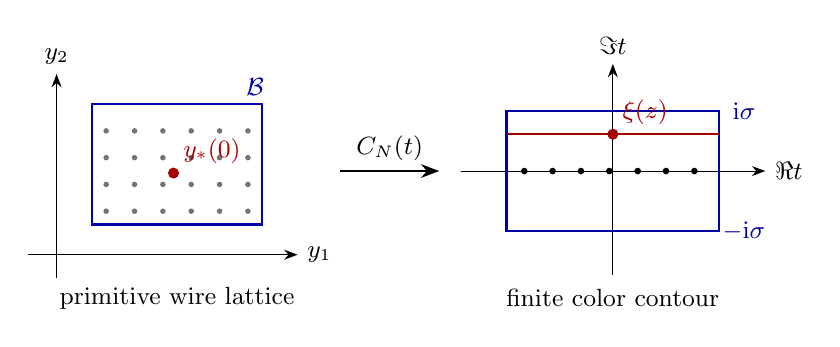
\begin{tikzpicture}[x=0.9cm,y=0.85cm,>=Stealth,font=\small]
\begin{scope}
 \draw[->](-.4,0)--(3.4,0) node[right]{$y_1$};
 \draw[->](0,-.35)--(0,2.7) node[above]{$y_2$};
 \draw[blue!65!black,thick](.5,.45)rectangle(2.9,2.25);
 \foreach \x in {.7,1.1,1.5,1.9,2.3,2.7}
  \foreach \y in {.65,1.05,1.45,1.85}
    \fill[black!55](\x,\y)circle(1pt);
 \fill[red!65!black](1.65,1.22)circle(2pt)
    node[above right]{$y_*(0)$};
 \node at(1.7,-.65){primitive wire lattice};
 \node[blue!65!black]at(2.8,2.5){$\mathcal B$};
\end{scope}
\draw[->,thick](4,1.25)--(5.4,1.25)
 node[midway,above]{$C_N(t)$};
\begin{scope}[shift={(6.2,0)}]
 \draw[->](-.5,1.25)--(3.8,1.25)node[right]{$\Re t$};
 \draw[->](1.65,-.3)--(1.65,2.85)node[above]{$\Im t$};
 \draw[blue!65!black,thick](.15,.35)--(3.15,.35)--(3.15,2.15)--(.15,2.15)--cycle;
 \foreach \x in {.4,.8,1.2,1.6,2,2.4,2.8}
   \fill(\x,1.25)circle(1.2pt);
 \draw[red!65!black,thick](.15,1.8)--(3.15,1.8);
 \fill[red!65!black](1.65,1.8)circle(2pt)
   node[above right]{$\xi(z)$};
 \node at(1.65,-.65){finite color contour};
 \node[blue!65!black]at(3.5,.35){$-\ii\sigma$};
 \node[blue!65!black]at(3.5,2.15){$\ii\sigma$};
\end{scope}
\end{tikzpicture}

 \caption{The two finite lattices in the proof. The wire indices determine the exact finite function $C_N(t)$; each affine wire retains its integer offset. Its color samples are then summed to the even Fourier polynomial $\mathcal F_N(z)$. The horizontal contour moves are made only after an exact residue representation and an exponentially accurate wire interpolation. The outer rectangle retains all its connecting sides.}\label{ca:two-lattices}
\end{figure}

\section{Full integer powers and the entire filling functional}\label{ca:filling}

A retained half twist can be left in the source or included in the full crossing power. We use the latter exact description here: each original disk carries $R^{n_\ell}$ with $n_\ell=\epsilon_\ell-2p_\ell$, expanded into ordinary circles. The following calculation treats odd and even $n$, including negative $n$. Thus no endpoint parity is changed by the rearrangement.

\subsection{The full Hermite data and their finite Fourier transform}

Write $\mathscr P_N(\sigma)=2T_N(\sigma/2)+2$ for the monic root polynomial and
\[
 w_k=q^{2k+1},\qquad c_k=w_k+w_k^{-1},\qquad 0\le k\le d.
\]
Its repeated roots remain repeated. In the full quotient
$\mathbb C[\sigma]/(\mathscr P_N)$ the normalized crossing $r_N=\kappa^{-1}R$ has
\begin{equation}\label{ca:crossing-data}
 r_N(c_k)=(-1)^kq^{k(k+1)},\qquad
 (w\partial_w)r_N(w+w^{-1})\big|_{w=w_k}
      =-\tfrac12(d-2k)r_N(c_k).
\end{equation}
The second formula is the derivative at the double nodes; at the odd simple node $w_k=-1$ it is zero and imposes no extra normal. These are the full crossing data proved in \cite[Proposition 5.1]{Finite} and \cite[equation (4.8)]{Newton}. Every value is nonzero. Hence the crossing is a unit in the full quotient, and all integer powers, including negative ones, are defined there.

Let $f_{N,n}$ be the unique representative of degree at most $d$ of $r_N^n$.
Put
\[
\begin{gathered}
 h_k=(-1)^{nk}q^{nk(k+1)},\qquad
 d_k=-\frac n2(d-2k)h_k,\\
 H_a=\frac1N\sum_{k=0}^d h_kw_k^{-a},\qquad
 D_a=\frac1N\sum_{k=0}^d d_kw_k^{-a}.
\end{gathered}
\]
Here $d_k$ is a normal datum, not the level shift $d$.
For $\mathsf C_a(w+w^{-1})=w^a+w^{-a}$, write
$f_{N,n}=a_0+\sum_{a=1}^d a_a\mathsf C_a$. Discrete Fourier inversion on $w_k^N=-1$ gives
\begin{equation}\label{ca:Hermite-inverse}
 a_0=H_0,\qquad
 a_a=\frac{D_a+(N-a)H_a}{N}\quad(1\le a<N).
\end{equation}
Indeed the value and normal equations are
$H_a=a_a-a_{N-a}$ and
$D_a=a\,a_a+(N-a)a_{N-a}$. When $N$ is even and $a=N/2$, the first equation is identically zero and the second still recovers the coefficient. At odd $N$ the simple node has only its value. These equations therefore recover the whole quotient, not just its distinct-root values.

Since
$\mathsf C_a=U_a(\sigma/2)-U_{a-2}(\sigma/2)$ for $a\ge1$,
with $U_{-1}=0$, set $a_N=a_{N+1}=0$ and
\begin{equation}\label{ca:beta}
 \beta_j^{n/2}=(-1)^j(a_j-a_{j+2}),\qquad0\le j<N.
\end{equation}
The superscript is a parameter and need not be an integer. The actual circles
$L_{j+1}=(-1)^jU_j(\sigma/2)$ satisfy the exact physical identity
\begin{equation}\label{ca:crossing-split}
 R^n=\kappa^n\sum_{j=0}^{d}\beta_j^{n/2}L_{j+1},
 \qquad
 \sum_{j=0}^{d}|\beta_j^{n/2}|
       \le 2N(1+|n|/2).
\end{equation}
For the bound use $|H_a|\le1$, $|D_a|\le |n|d/2$ in
\eqref{ca:Hermite-inverse}, then sum the two coefficient contributions in
\eqref{ca:beta}. The equality is first an identity in the one local pair algebra and then evaluated in the diagram. Distinct physical boxes have not been commuted.

\subsection{The midpoint identity, including odd physical powers}

Let $C_N(t)$ be the even strict pure corridor of
Theorem~\ref{ca:strict-pure}, with one variable for the moment, and let
$\mathcal F_N(z)=\sum_{|h|\le H_N^{\rm cut}}C_N(h/N)e^{2\pi\ii hz}$.
Put
\[
 z_k=\frac{k+1/2}{N}-\frac12,\qquad
 U_N(z)=e^{\pi\ii nNz^2}\sinh(2\pi\ii z)\mathcal F_N(z).
\]
On the actual midpoint grid, for every integer $n$,
\begin{equation}\label{ca:chirp}
 h_k=\kappa^{-n/2}e^{\pi\ii nNz_k^2},\qquad
 d_k=nNz_kh_k.
\end{equation}
For example, the first equality follows by writing
$(-1)^k=e^{-\pi\ii k}$ at integer $k$ and using
$-k+k(k+1)/N=Nz_k^2-d^2/(4N)$. This fixes the fractional power
$\kappa^{n/2}=e^{\pi\ii n d^2/(4N)}$ without a branch convention.

Substitute \eqref{ca:chirp} into \eqref{ca:Hermite-inverse}--\eqref{ca:beta}. Pairing the $h$ and $-h$ terms gives
\begin{equation}\label{ca:midpoint}
 \sum_{h=0}^{H_N^{\rm cut}}\beta_{N-h-1}^{n/2}C_N(h/N)
 =\frac{(-1)^d\kappa^{-n/2}}{2\pi\ii N^2}
      \sum_{k=0}^{N-1}U_N'(z_k).
\end{equation}
To see the endpoint multiplicity directly, for $h\ge1$ the summand before this pairing is
\[
 \frac{2(-1)^d\kappa^{-n/2}}{N^2}
 \sum_k e^{\pi\ii nNz_k^2+2\pi\ii h z_k}
 \{(nNz_k+h)\sinh(2\pi\ii z_k)+\cosh(2\pi\ii z_k)\}.
\]
For $h=0$ it is half this expression. The symmetric Fourier polynomial has two terms at $h\ne0$ and one at zero, exactly as required by \eqref{ca:midpoint}. Its derivative includes the original normal term $nNz_k$; omitting that term would give a different functional.

Both endpoint values of $U_N$ vanish, and
$U_N'(1/2)=U_N'(-1/2)$. Its periodically extended derivative is continuous and piecewise smooth. Two integrations by parts give an absolutely summable Fourier series for each fixed $N$. Midpoint selection and a further integration by parts yield
\begin{equation}\label{ca:charge-one}
 (-1)^d\kappa^{-n/2}
 \sum_{m\ne0}(-1)^{md}m
 \int_{-1/2}^{1/2}
 e^{\pi\ii nNz^2-2\pi\ii mNz}
 \sinh(2\pi\ii z)\mathcal F_N(z)\dd z.
\end{equation}
The zero charge is absent because the original endpoint values vanish. This is an exact convergent identity at each $N$, not yet an estimate of a tail as $N$ grows.

Apply this identity in all $b$ color registers and restore
$\kappa^{\sum n_\ell}$ from \eqref{ca:crossing-split}. Change $m_\ell$ to $-\ell_\ell$ and use $\sinh(2\pi\ii z)=\ii\sin(2\pi z)$. The resulting corridor evaluation is
\begin{equation}\label{ca:generic-period}
 (-1)^{bd}\mathcal I_N(\mathbf n),
\end{equation}
where, with $I=[-1/2,1/2]$,
\begin{align}
 \mathcal I_N(\mathbf n)
 ={}&\kappa^{\frac12\sum n_\ell}(-\ii)^b
 \sum_{\ell\in(\mathbb Z\setminus\{0\})^b}
       \left(\prod_j\ell_j\right)(-1)^{(N+1)\sum_j\ell_j}\notag\\
 &\quad\times\int_{I^b}\mathcal F_N(z)
       \prod_j\sin(2\pi z_j)
       e^{N\{\pi\ii\sum_jn_jz_j^2+
                         2\pi\ii\sum_j\ell_jz_j\}}\dd z.\label{ca:period}
\end{align}
This is precisely the normalization in \cite[equation (1.6)]{Filling}; the definition \eqref{ca:period} fixes it independently of that equation number.

Before using any asymptotic theorem, \eqref{ca:crossing-split} and
Theorem~\ref{ca:strict-pure} show that replacing the full physical source by this corridor changes its filled value by at most
\begin{equation}\label{ca:filled-error}
 \prod_j2N(1+|n_j|/2)\ e^{N(F_0-\gamma_*)}
\end{equation}
for a fixed $\gamma_*>0$. The source error and macroscopic-color errors were bounded before extending colors by evenness. Thus an alias is never silently folded as though it were even. For fixed $\mathbf n$, the displayed prefactor is polynomial in $N$.

\subsection{Application to the whole sum and the primitive action}

Proposition~\ref{ca:Fourier-theorem} verifies every analytic input of
\cite[Theorem 1.1]{Filling} for this exact polynomial. Its separate degree is at most $d$. In the notation of that theorem take
\[
 \alpha=3/2+b/2,\qquad \varepsilon_N=1,\qquad
 A_N=\Psi_0,\qquad a_N=B,\qquad c_j=\pi/X_j.
\]
The action is real on the real polydisk; the global gap is for the whole polynomial on the entire shared cube and a fixed complex strip. Polynomial factors in \eqref{ca:Fourier-global} are absorbed into half its strict gap. Thus the theorem controls all distant integer charges, their paired endpoint currents, and all remaining finite nonlocal charges. These controls are part of the imported whole-sum theorem, not an assertion that convergence of \eqref{ca:period} alone suffices.

Its nonzero leading expression, multiplied by \eqref{ca:generic-period}, has parity factor
$(-1)^{bd+(N+1)b}=1$. Its power of $N$ is
$\alpha-b/2=3/2$. The local phase and amplitude are independent of $N$ here, so the theorem's finite critical action is exactly $S_{\mathbf n}$, not merely a sequence converging to it. It gives
\eqref{ca:asymptotic}--\eqref{ca:D} for the corridor. Also
$F_0-\Re S_{\mathbf n}=O(\sum n_j^{-2})$ with no ratio constraint.
Increase a fixed threshold on the independent $|n_j|$ until this loss is smaller than $\gamma_*/2$. Then \eqref{ca:filled-error} is exponentially below the nonzero leading term. This proves the same relative asymptotic for the whole original evaluation.

It remains to identify its action with the original marked filling,
especially when a physical power is odd. We use a classical shear
defined at every strict leaf, not a signed quantum asymptotic at
that leaf. For $0<x<1/2$ and $v=g_t(x,t)$ put
\[
 \chi=t-\frac{\epsilon}{2\pi\ii}v,\qquad
 f_\epsilon^{\rm cl}(x,\chi)
        =g(x,t)-\frac{\epsilon}{4\pi\ii}v^2.
\]
At zero its change of parameter has derivative
$1-\epsilon\ii\cot(\pi x)\ne0$, so it is locally invertible.
Direct differentiation gives
$\dd f_\epsilon^{\rm cl}=g_x\,\dd x+v\,\dd\chi$.
These are exactly the mixed-pyramid potential and the
primitive retained-half-twist shear of
\cite[Section 6, equations (6.1)--(6.5)]{StrictGeometry};
the normalization is $J(0)=0$ and $f_\epsilon^{\rm cl}(x,0)=g(x,0)$.
Their construction is classical and includes $x=1/4$.
On the high-index interval they agree with
Proposition~\ref{ca:shear}, but that agreement is not needed here.

Sum these functions and the unchanged gate actions and eliminate
the stationary wires. Denote the resulting classical action by
$\Phi_\epsilon^{\rm cl}$. The differential just computed shows that
its wire derivatives are precisely the pure wire derivatives at
the changed colors. Hence the pure stationary wires are also
stationary for this sheared action. Its Hessian in those wires
is invertible near zero, so they are the same local branch.
The envelope rule and the local formula give the exact identities
\begin{align}
 \chi_j&=t_j-\frac{\epsilon_j}{2\pi\ii}
                             \partial_{t_j}\Phi_0(t),\notag\\
 \Phi_\epsilon^{\rm cl}(\chi)
   &=\Phi_0(t)
       -\sum_j\frac{\epsilon_j}{4\pi\ii}
                         [\partial_{t_j}\Phi_0(t)]^2.\label{ca:global-shear}
\end{align}
The right side is an identity of functions, not merely of their
derivatives. It fixes the additive constant and every
color-dependent term. By its construction it is the cell potential
of \cite[Theorem 1.3]{StrictGeometry}, for the same original
expression, disk framings and retained half twists.

For the Fourier Legendre functions, \eqref{ca:global-shear} gives
\begin{equation}\label{ca:Legendre-shear}
 \Psi_\epsilon^{\rm cl}(z)=\Psi_0(z)+\pi\ii\sum_j\epsilon_jz_j^2,
 \qquad \chi=t+\epsilon z,
 \quad \nabla\Phi_0(t)=-2\pi\ii z.
\end{equation}
Let $z=z_{\mathbf n}$ be the charge-one critical point. Its equation is
$\xi(z)+\mathbf n z+\mathbf1=0$, componentwise. By evenness put
$z_g=-z$ and $t_g=-\xi(z)$; then
$t_g=\mathbf1-\mathbf n z_g$. Therefore
\[
 \chi=t_g+\epsilon z_g=\mathbf1+2\mathbf p z_g.
\]
Substitution into the Legendre expression gives exactly
\begin{align}
 S_{\mathbf n}
 &=\Psi_0(z_g)+\pi\ii\sum_jn_j z_{g,j}^2
                        -2\pi\ii\sum_j z_{g,j}\notag\\
 &=\Phi_\epsilon^{\rm cl}(\chi)
       +\frac{\pi\ii}{2}\sum_j\frac{(\chi_j-1)^2}{p_j}.
 \label{ca:classical-action}
\end{align}
The primitive similarity logarithms in that theorem are
\[
 U_j=-2\pi\ii\chi_j,\qquad
 V_j=-2\partial_j\Phi_\epsilon^{\rm cl}
       =4\pi\ii z_{g,j}.
\]
Consequently $U_j+p_jV_j=-2\pi\ii$ exactly, with the original
integer $p_j$. These equations also show that $\chi$ is critical
for the final expression in \eqref{ca:classical-action}.
Since $z_{\mathbf n}=O(\max_j|n_j|^{-1})$ and
$\xi(z)=O(\|z\|)$, the formula $\chi=t_g+\epsilon z_g$
shows that $\chi$ tends to zero independently of the ratios
of the filling integers. Local uniqueness in
\cite[Theorem 1.3]{StrictGeometry} therefore identifies it with
the primitive filling branch through the oriented complete metric.
No uniqueness of the full character variety is used.
That theorem keeps the original full group relations and main
parabolic cusps, proves smooth completion on the actual filled
exterior, and compares the same positive cell chain with the
metric fundamental chain. Its conclusion is the absolute equality
$\Vol(S^3\setminus K_{\epsilon,\mathbf p})
=2\pi\Re S_{\mathbf n}$.
The knot test in Section~\ref{ca:intro} is what makes this
filled main link a knot.

Take $P_0$ larger than the geometric threshold and large enough that
$|n_j|=|\epsilon_j-2p_j|$ exceeds the source and whole-period thresholds. The equality holds for every fixed signed tuple beyond it. Finally the framing factor and all powers of $\kappa$ have modulus one; the Gaussian coefficient is nonzero. Taking logarithms proves \eqref{ca:volume} and completes the proof of Theorem~\ref{ca:main}.


\section{Finite reproduction and the use of the result}\label{ca:reproduction}
The accompanying Python program \texttt{check.py} uses only the standard library. Run
\[
 \texttt{python3 -I papers/conway-asymptotics/check.py}
\]
from the repository root, optionally adding
\texttt{--output /path/to/directory}. It removes a previous summary before validation and records its source hashes before and after the run.

For levels $2$ through $12$, over two finite fields containing a primitive $8N$th root at each level, the program constructs the crossing from its normalized Newton polynomial. Ordinary polynomial division then forms its powers $-3,-2,-1,0,1,2,3$, using the extended Euclidean algorithm for negative powers. These polynomials are compared with the independently formed value and angular-normal data, their Fourier--Hermite inversion, and their expansion in ordinary circles. Three explicit even corridor sequences in each case test the midpoint formula, including its $h=0$ weight. There are $154$ integer-power cases and $462$ midpoint cases. The test does not assume a prime level or discard an odd simple node.

The all-level algebraic argument is in Section~\ref{ca:filling}; the finite checks can detect transcription and normalization errors but are not its proof. They do not test analytic continuation, contour estimates or metric completion. The strict volume proof uses exact pure factorial interpolation, the strict variational theorem, the whole complementary-source bounds, the two finite-contour arguments, the whole-charge theorem and the marked metric theorem. The signed recurrence supplies the separate completed-root packet theorem. Theorem~\ref{ca:main} concerns each fixed strict presentation and independently sufficiently long fixed fillings. It does not assert a result for boundary-only presentations or for constructions that grow with $N$.

\begin{thebibliography}{9}
\bibitem{Newton}\emph{Newton coefficients and positive sources for Conway tangles}.
Companion paper, \href{https://sashakolpakov.github.io/murakamis_dream/papers/newton-tangles.pdf}{repository edition}.
\bibitem{Profiles}\emph{Stationary profiles of strict Newton trees}.
Companion paper, \href{https://sashakolpakov.github.io/murakamis_dream/papers/strict-newton-profiles.pdf}{repository edition}.
\bibitem{Bounds}\emph{Spectral estimates for Conway tangle sources}.
Companion paper, \href{https://sashakolpakov.github.io/murakamis_dream/papers/conway-source-bounds.pdf}{repository edition}.
\bibitem{Filling}\emph{Oscillatory filling sums with independently long twists}.
Companion paper, \href{https://sashakolpakov.github.io/murakamis_dream/papers/oscillatory-fillings.pdf}{repository edition}.
\bibitem{StrictGeometry}\emph{Marked geometry of strict Conway compositions}.
Companion paper, \href{https://sashakolpakov.github.io/murakamis_dream/papers/strict-conway-geometry.pdf}{repository edition}.
\bibitem{Finite}\emph{Finite spectral evaluation and uniform filling bounds}.
Companion paper, \href{https://sashakolpakov.github.io/murakamis_dream/papers/filling-bounds.pdf}{repository edition}.
\bibitem{DLMF} F. W. J. Olver et al., eds., \emph{NIST Digital Library of Mathematical Functions}, \href{https://dlmf.nist.gov/5.5}{\S5.5} and \href{https://dlmf.nist.gov/5.11}{\S5.11}.
\end{thebibliography}
\end{document}
